\problemname{Kaninhål}

I den nyss avslutade tävlingen Databävern \href{www.databavern.se}{(se hemsida)} fick
eleverna se ett exempel på djurens märkliga samspel:

En grupp med $N$ bävrar ska gå på promenad i skogen. De går på ett led efter
varandra, den ena bävern efter den andra. Men de busiga kaninerna har grävt en
massa hål utefter stigen som bävrarna går på.

Hålen är tillräckligt djupa för att ett visst antal bävrar ska falla i dem. När
hålet väl är fullt med bävrar kan de bakomvarande bävrarna passera ovanpå
bävrarna i hålet, tills slutligen den sista bävern i raden drar upp bävrarna ur
hålet, den översta först och den understa sist. Alltså, om vi har fem bävrar (5
4 3 2 1) som vandrar åt höger (nummer 1 går alltså först och nummer 5 sist i
ledet), och de kommer till ett hål där tre bävrar får plats, så skulle följande
hända:

\begin{figure}[ht!]
\centering
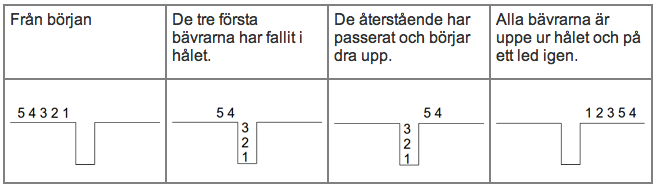
\includegraphics[width=0.7\textwidth]{kaninhol.png}
\caption{En illustration av ett kanin hål och hur bävrarna vandrar över hålet.}
\label{overflow}
\end{figure}

Tänk dig nu att kaninerna har gjort tre hål på vägen (vardera med ett djup
mellan $1$ och $N-1$). Skriv ett program som, givet hur raden ser ut efter att
bävrarna passerat alla hålen, beräknar djupet för varje hål.

\section*{Indata}

På första raden står ett heltal $N$, antalet bävrar, där $2 \leq N < 10$. På andra raden
står $N$ olika heltal, vardera mellan 1 och N. Dessa beskriver ordningen på
bävrarna när de passerat de tre kaninhålen. Från början är ordningen $N$, $N-1$,
$N-2,\ldots,1$. Observera att de vandrar åt höger, så bäver $1$ går först i ledet.

\section*{Utdata}

Tre heltal mellan $1$ och $N-1$, djupet på det första, andra respektive tredje
kaninhålet. Du kan förutsätta att det finns exakt en lösning för varje givet
testfall.
